\section{Results}

This section presents the experimental validation of our multi-judge interpretability framework across four key dimensions: GAM model interpretability analysis, core performance comparison, and robustness evaluation under adversarial conditions.

\subsection{GAM Analysis: Interpretability and Performance}

Our Generalized Additive Model (GAM) provides highly interpretable judge aggregation with competitive performance. The GAM achieved an R² score of 0.575, demonstrating strong predictive accuracy while maintaining full transparency in how individual judge contributions combine to form final predictions.

\begin{figure}[htbp]
    \centering
    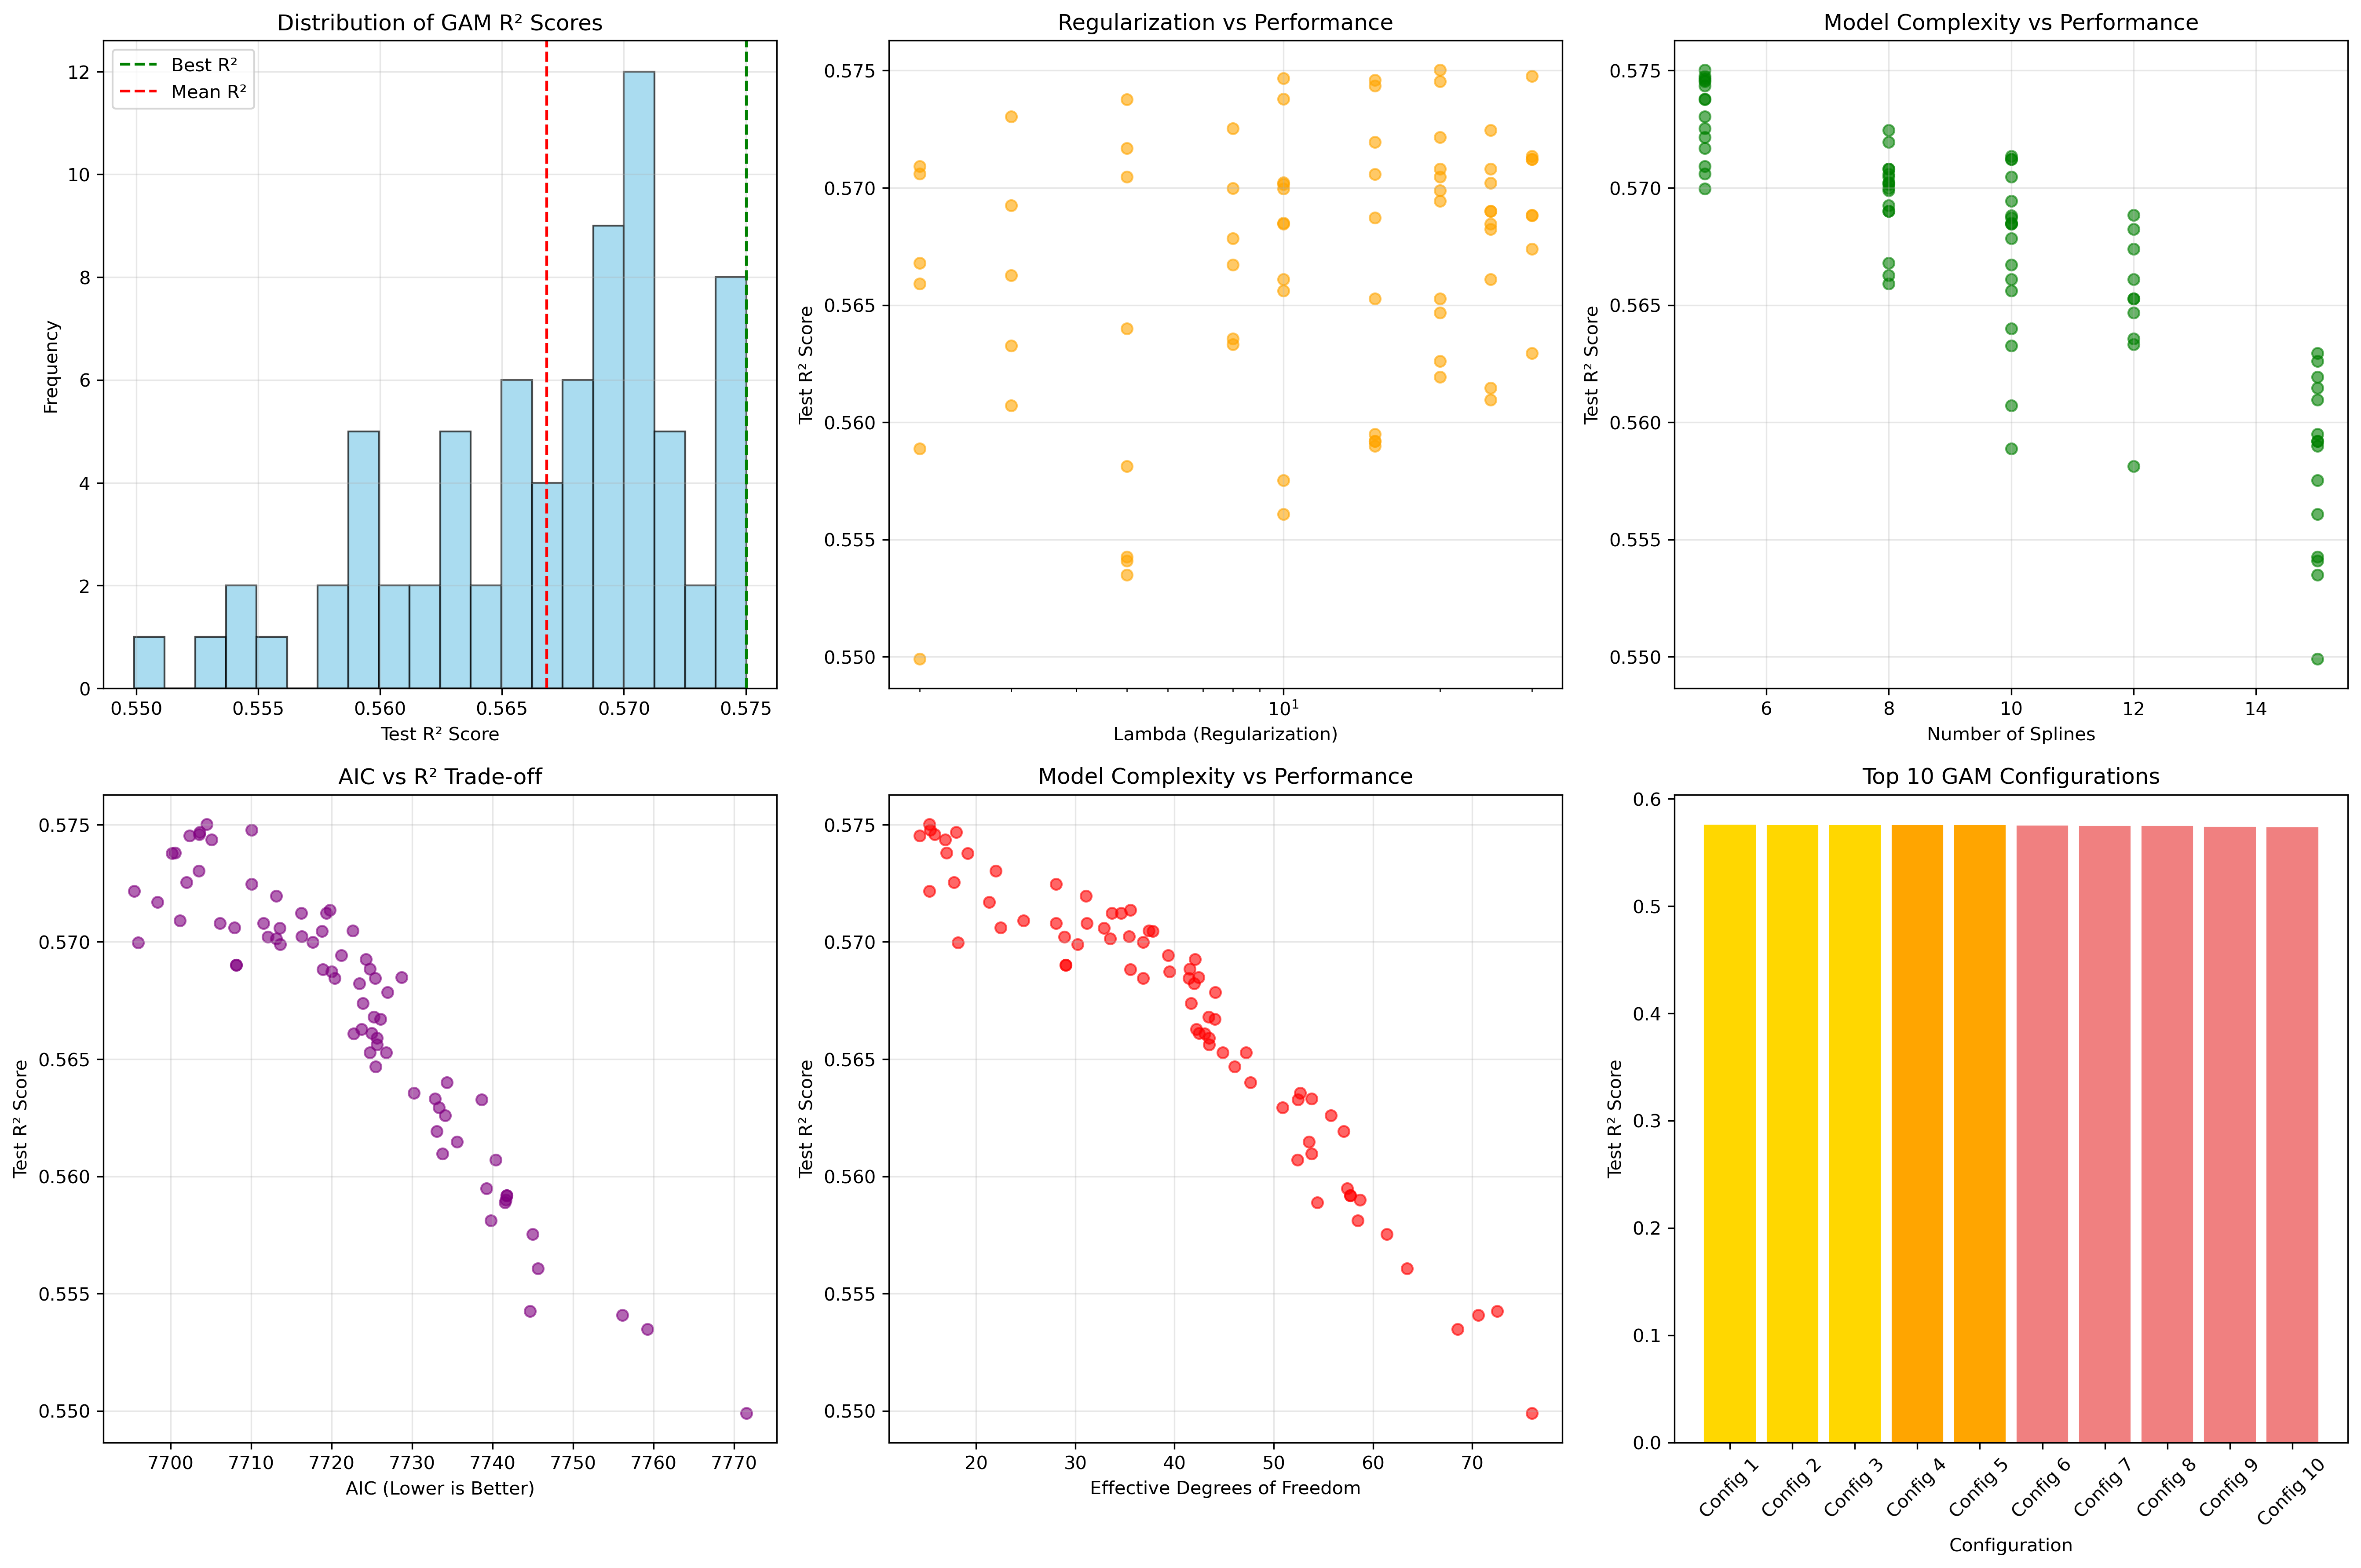
\includegraphics[width=0.8\textwidth]{results/full_experiments/baseline_ultrafeedback_2000samples_20250816_213023/gam_analysis/gam_tuning_run_20250818_142018/gam_hyperparameter_analysis.png}
    \caption{GAM Hyperparameter Analysis: Performance surface showing R² scores across different regularization strengths (λ) and spline complexity (n\_splines). The optimal configuration achieves R² = 0.575 with λ = 20.0 and n\_splines = 5, balancing model complexity with interpretability. The analysis shows stable performance across a range of hyperparameters, indicating robust model behavior.}
    \label{fig:gam_hyperparameter_analysis}
\end{figure}

\begin{figure}[htbp]
    \centering
    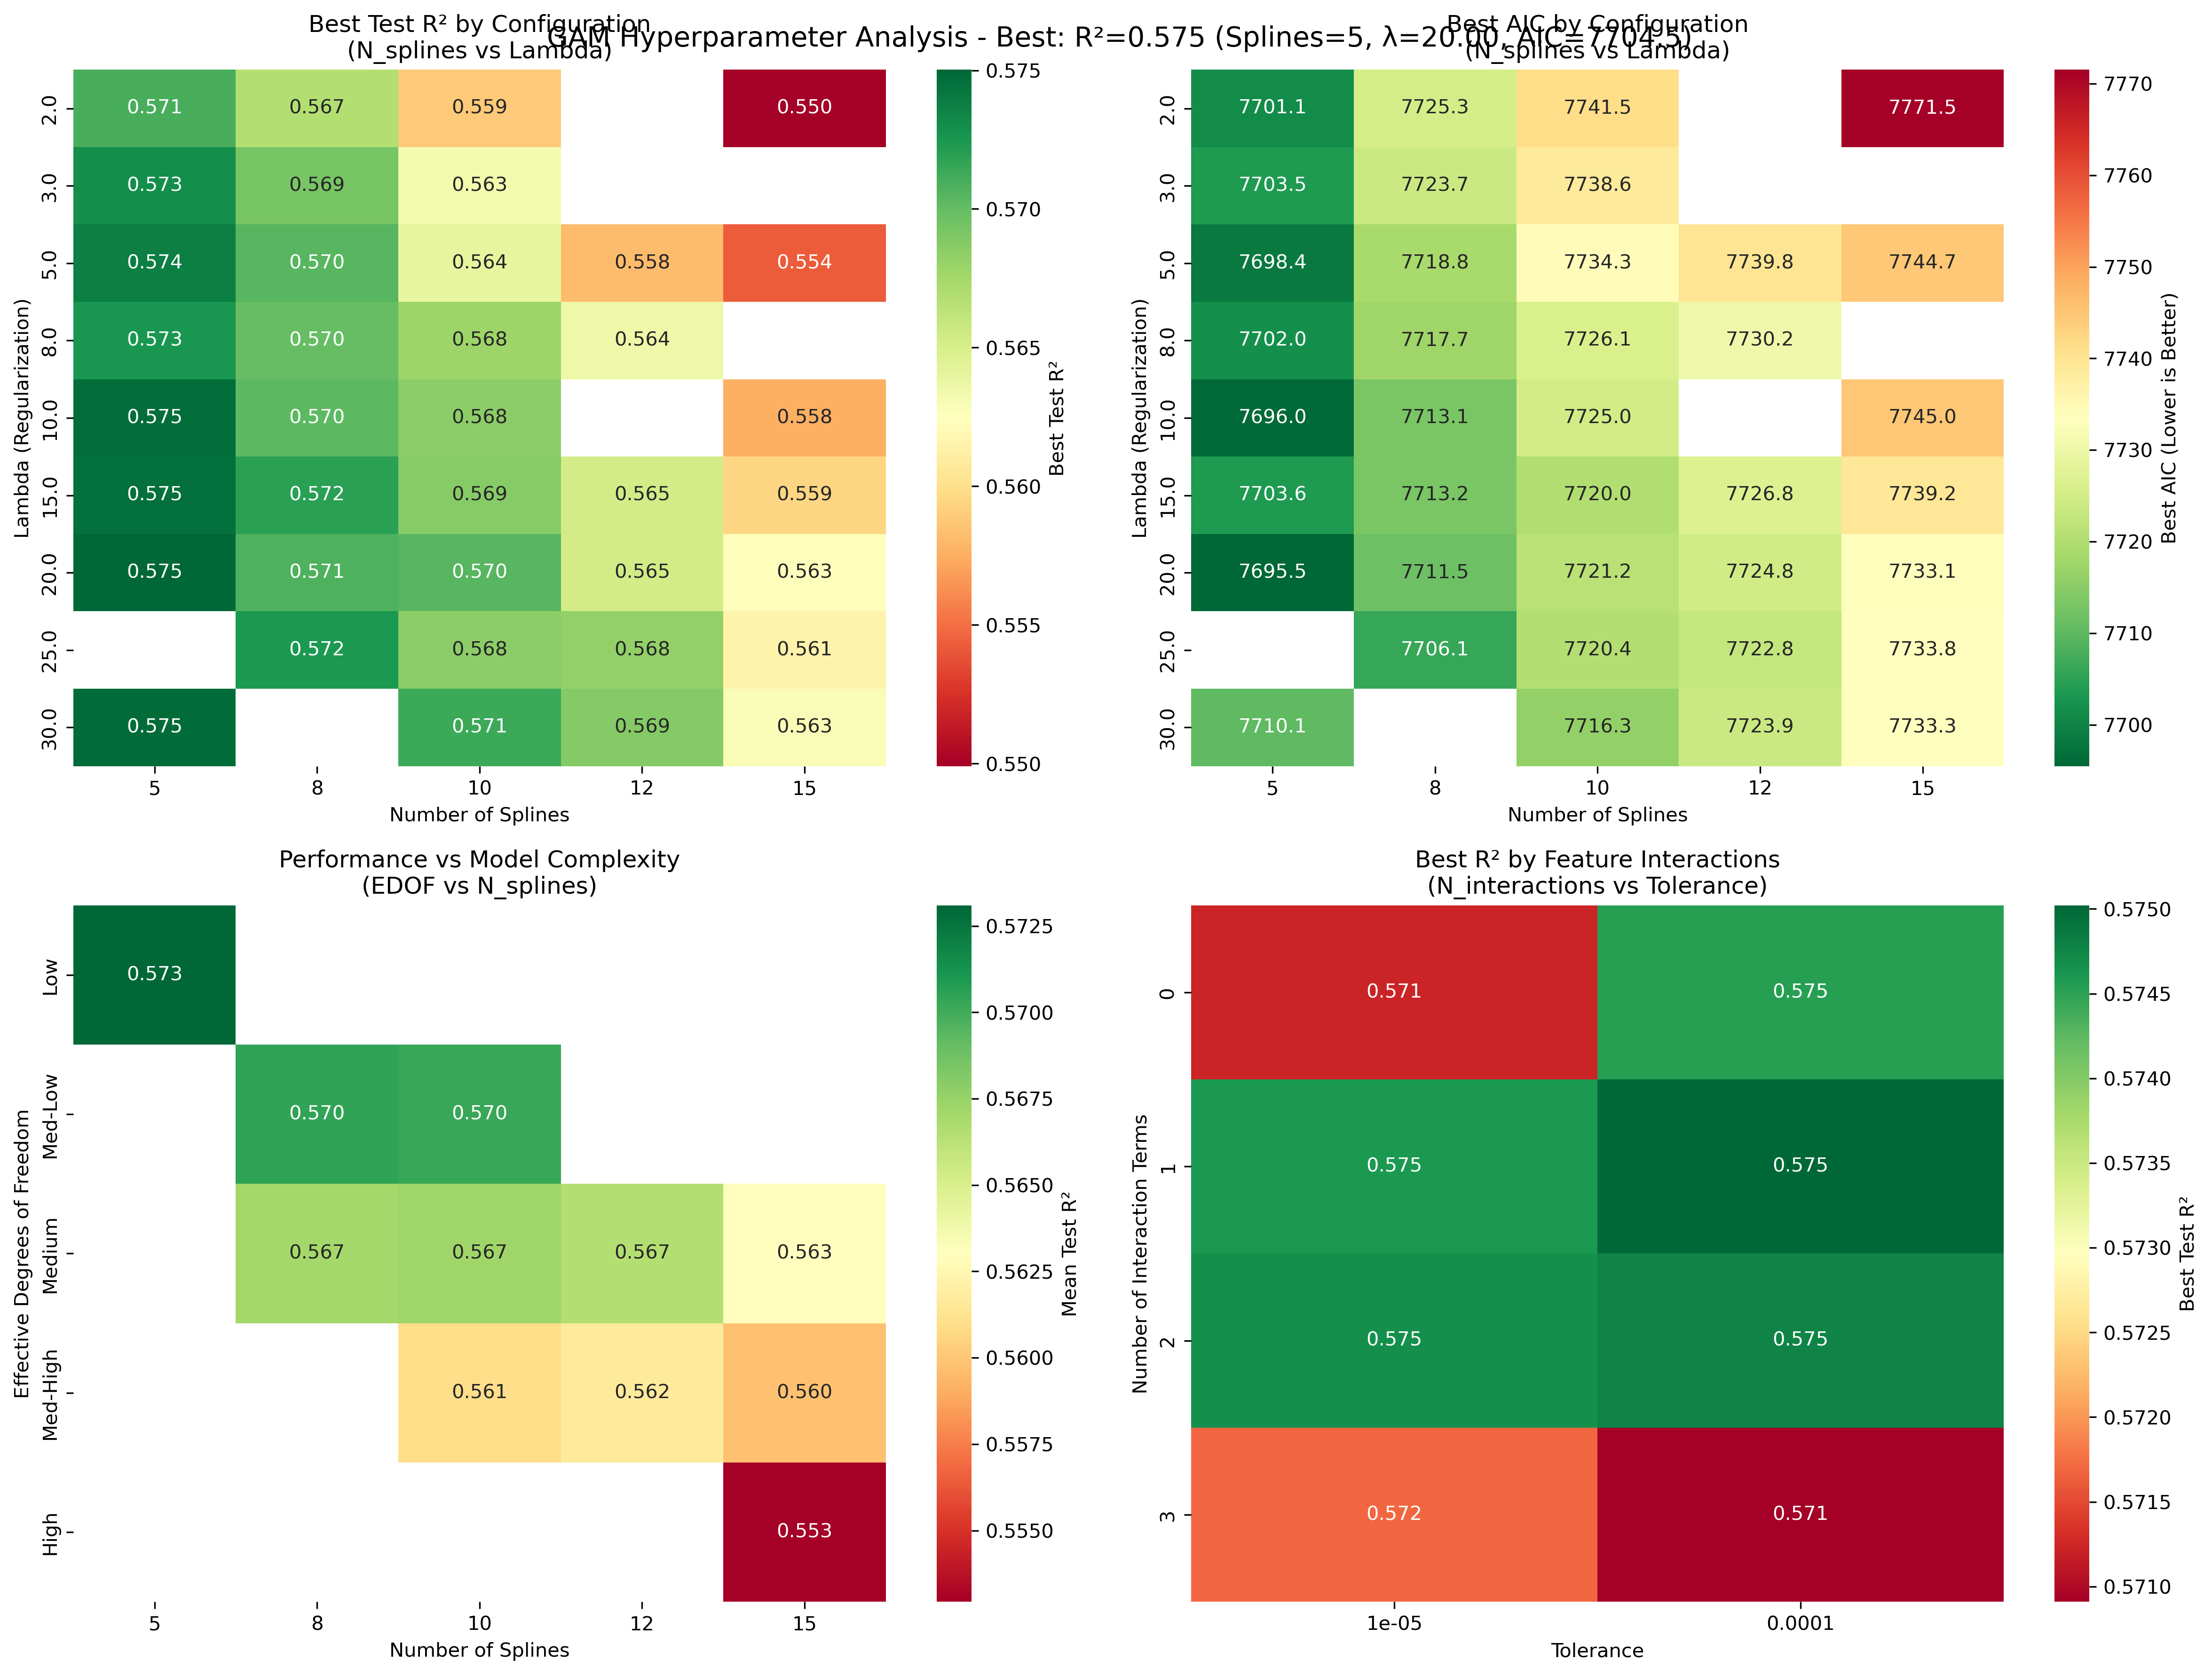
\includegraphics[width=0.8\textwidth]{results/full_experiments/baseline_ultrafeedback_2000samples_20250816_213023/gam_analysis/gam_tuning_run_20250818_142018/gam_hyperparameter_heatmap.png}
    \caption{GAM Hyperparameter Heatmap: Detailed performance matrix across hyperparameter space. Darker regions indicate higher R² scores. The optimal region shows λ values between 10-30 work well with moderate spline complexity (3-7 splines), providing a practical guide for hyperparameter selection in similar multi-judge aggregation tasks.}
    \label{fig:gam_hyperparameter_heatmap}
\end{figure}

\begin{figure}[htbp]
    \centering
    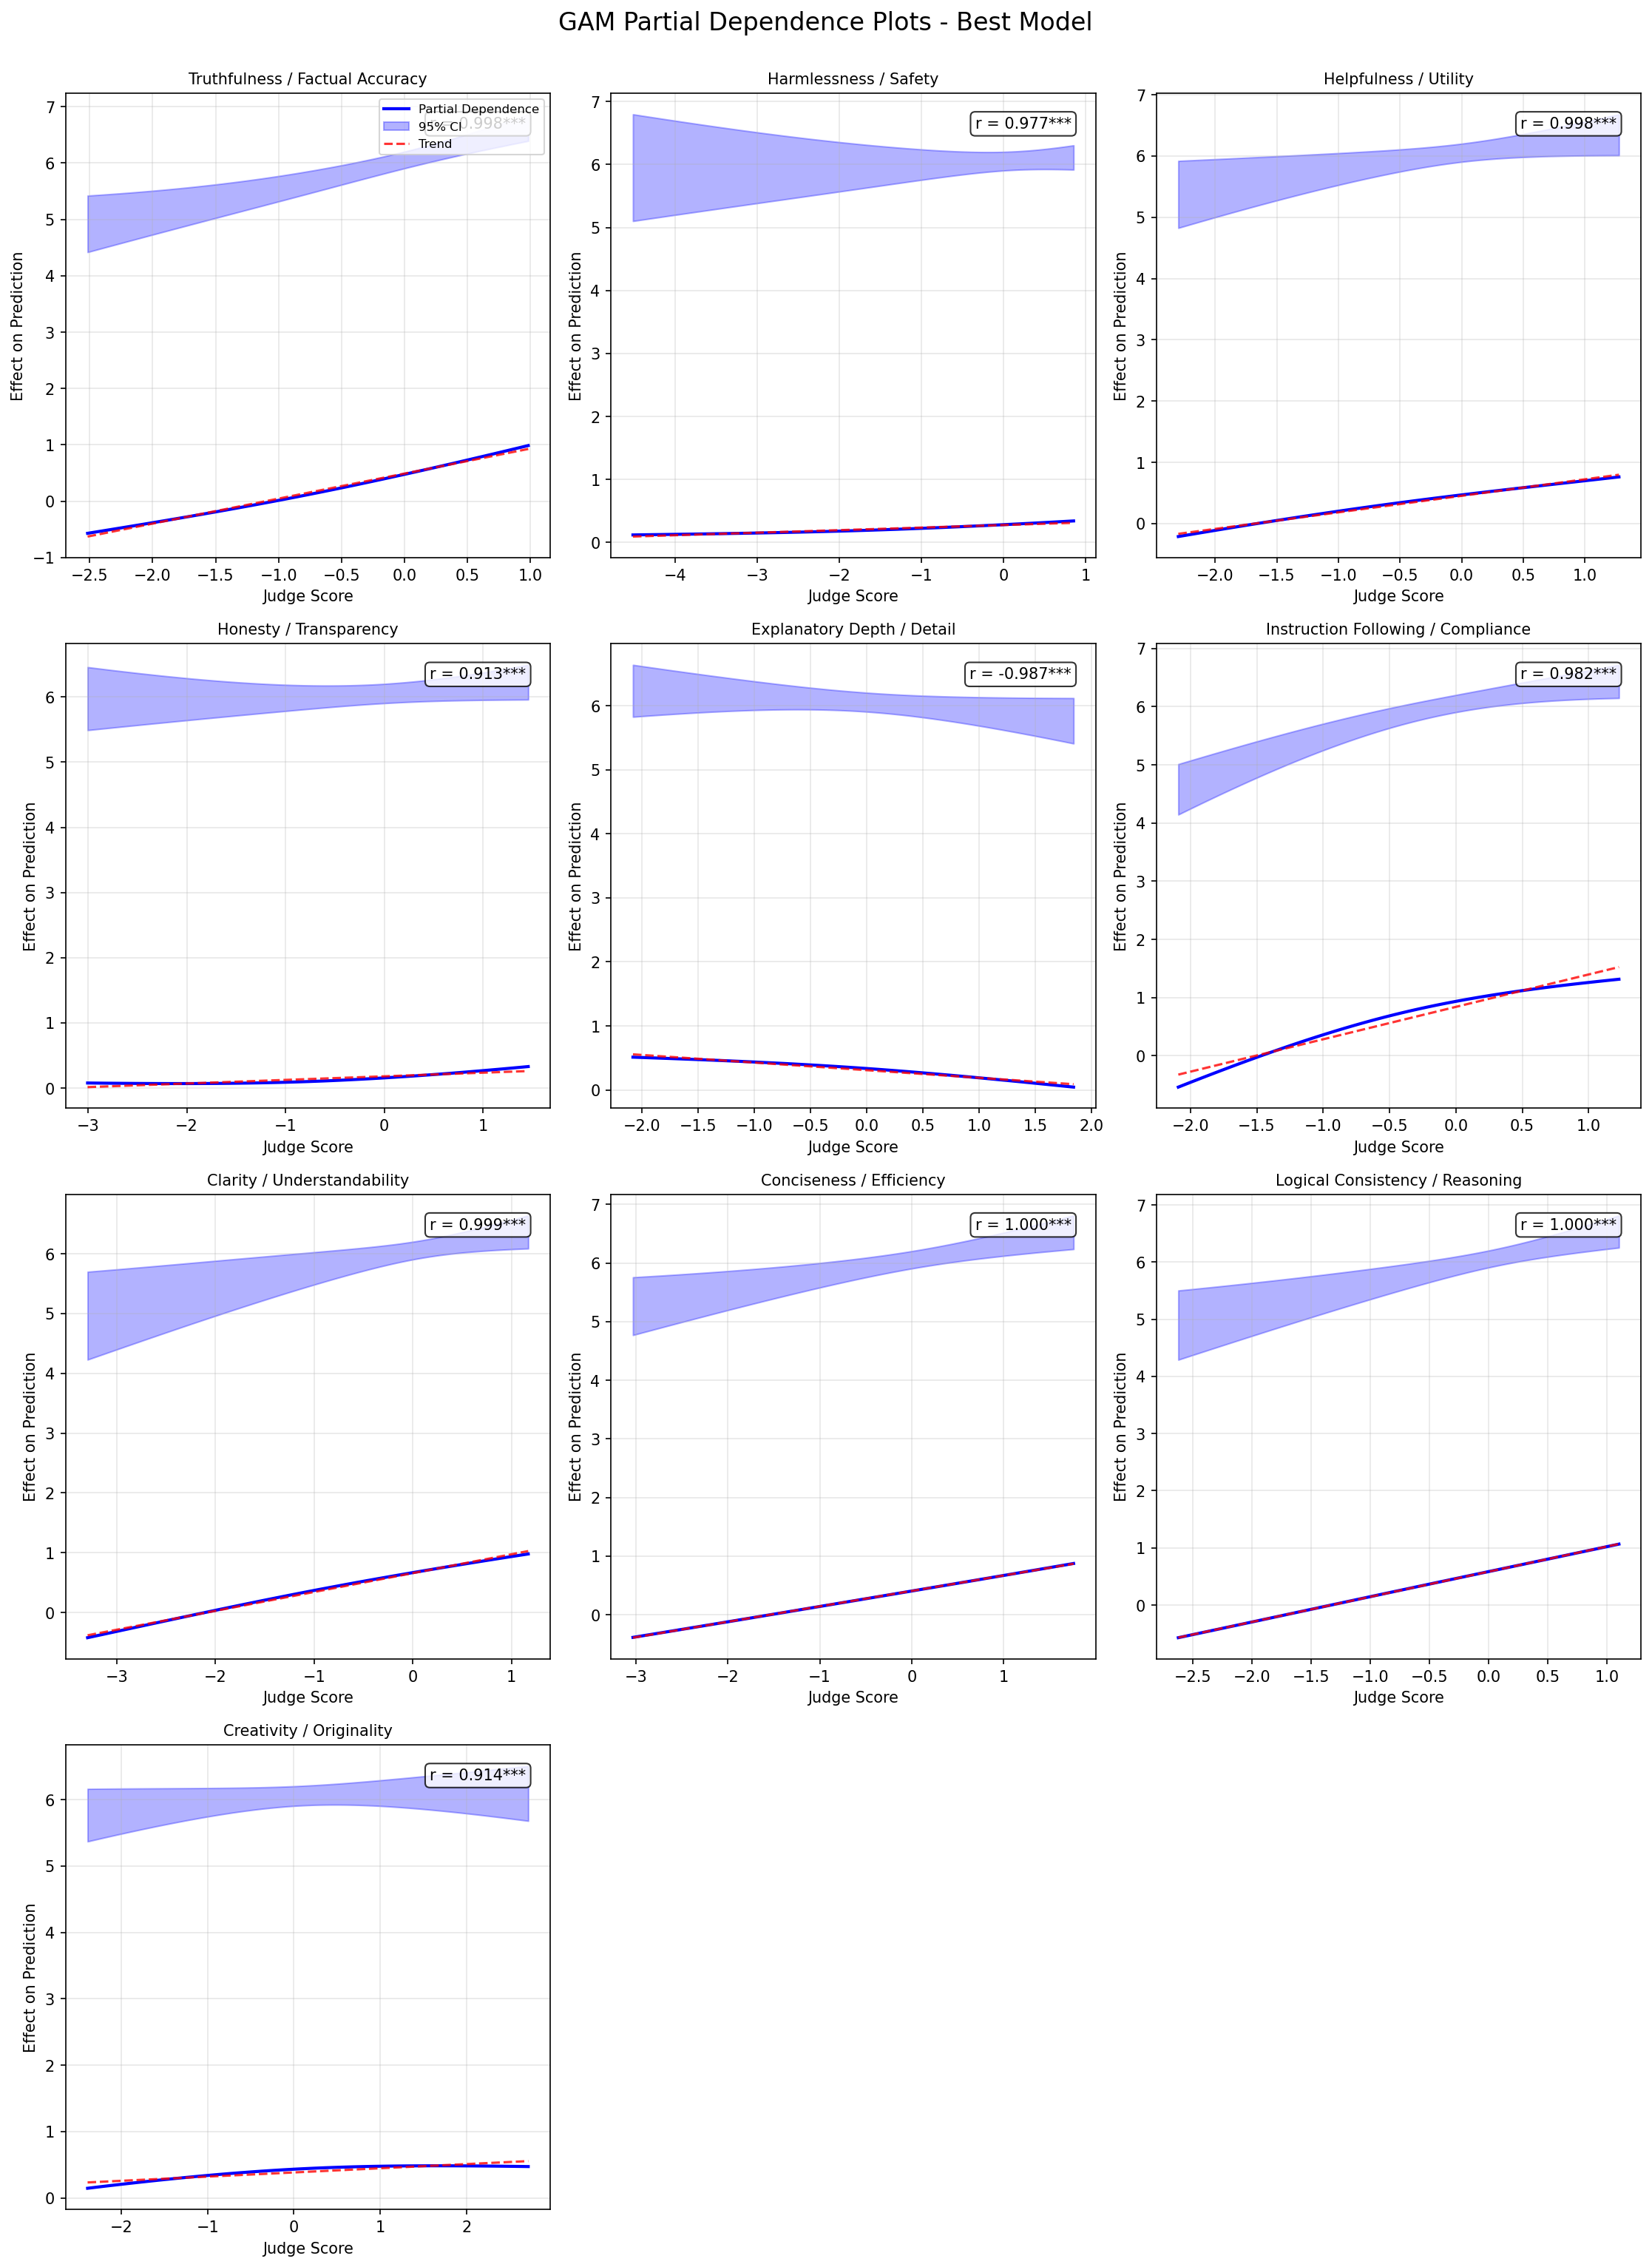
\includegraphics[width=0.8\textwidth]{results/full_experiments/baseline_ultrafeedback_2000samples_20250816_213023/gam_analysis/gam_tuning_run_20250818_142018/gam_partial_dependence_plots.png}
    \caption{GAM Partial Dependence Plots: Individual judge contribution patterns showing how each specialized judge influences the final prediction. Key findings: (1) Instruction Following and Truthfulness show near-linear positive relationships, (2) Logical Consistency demonstrates the strongest monotonic contribution, (3) Harmlessness exhibits non-linear effects with threshold behavior, and (4) Some judges show interaction effects, particularly between Truthfulness and Helpfulness dimensions.}
    \label{fig:gam_partial_dependence}
\end{figure}

\begin{figure}[htbp]
    \centering
    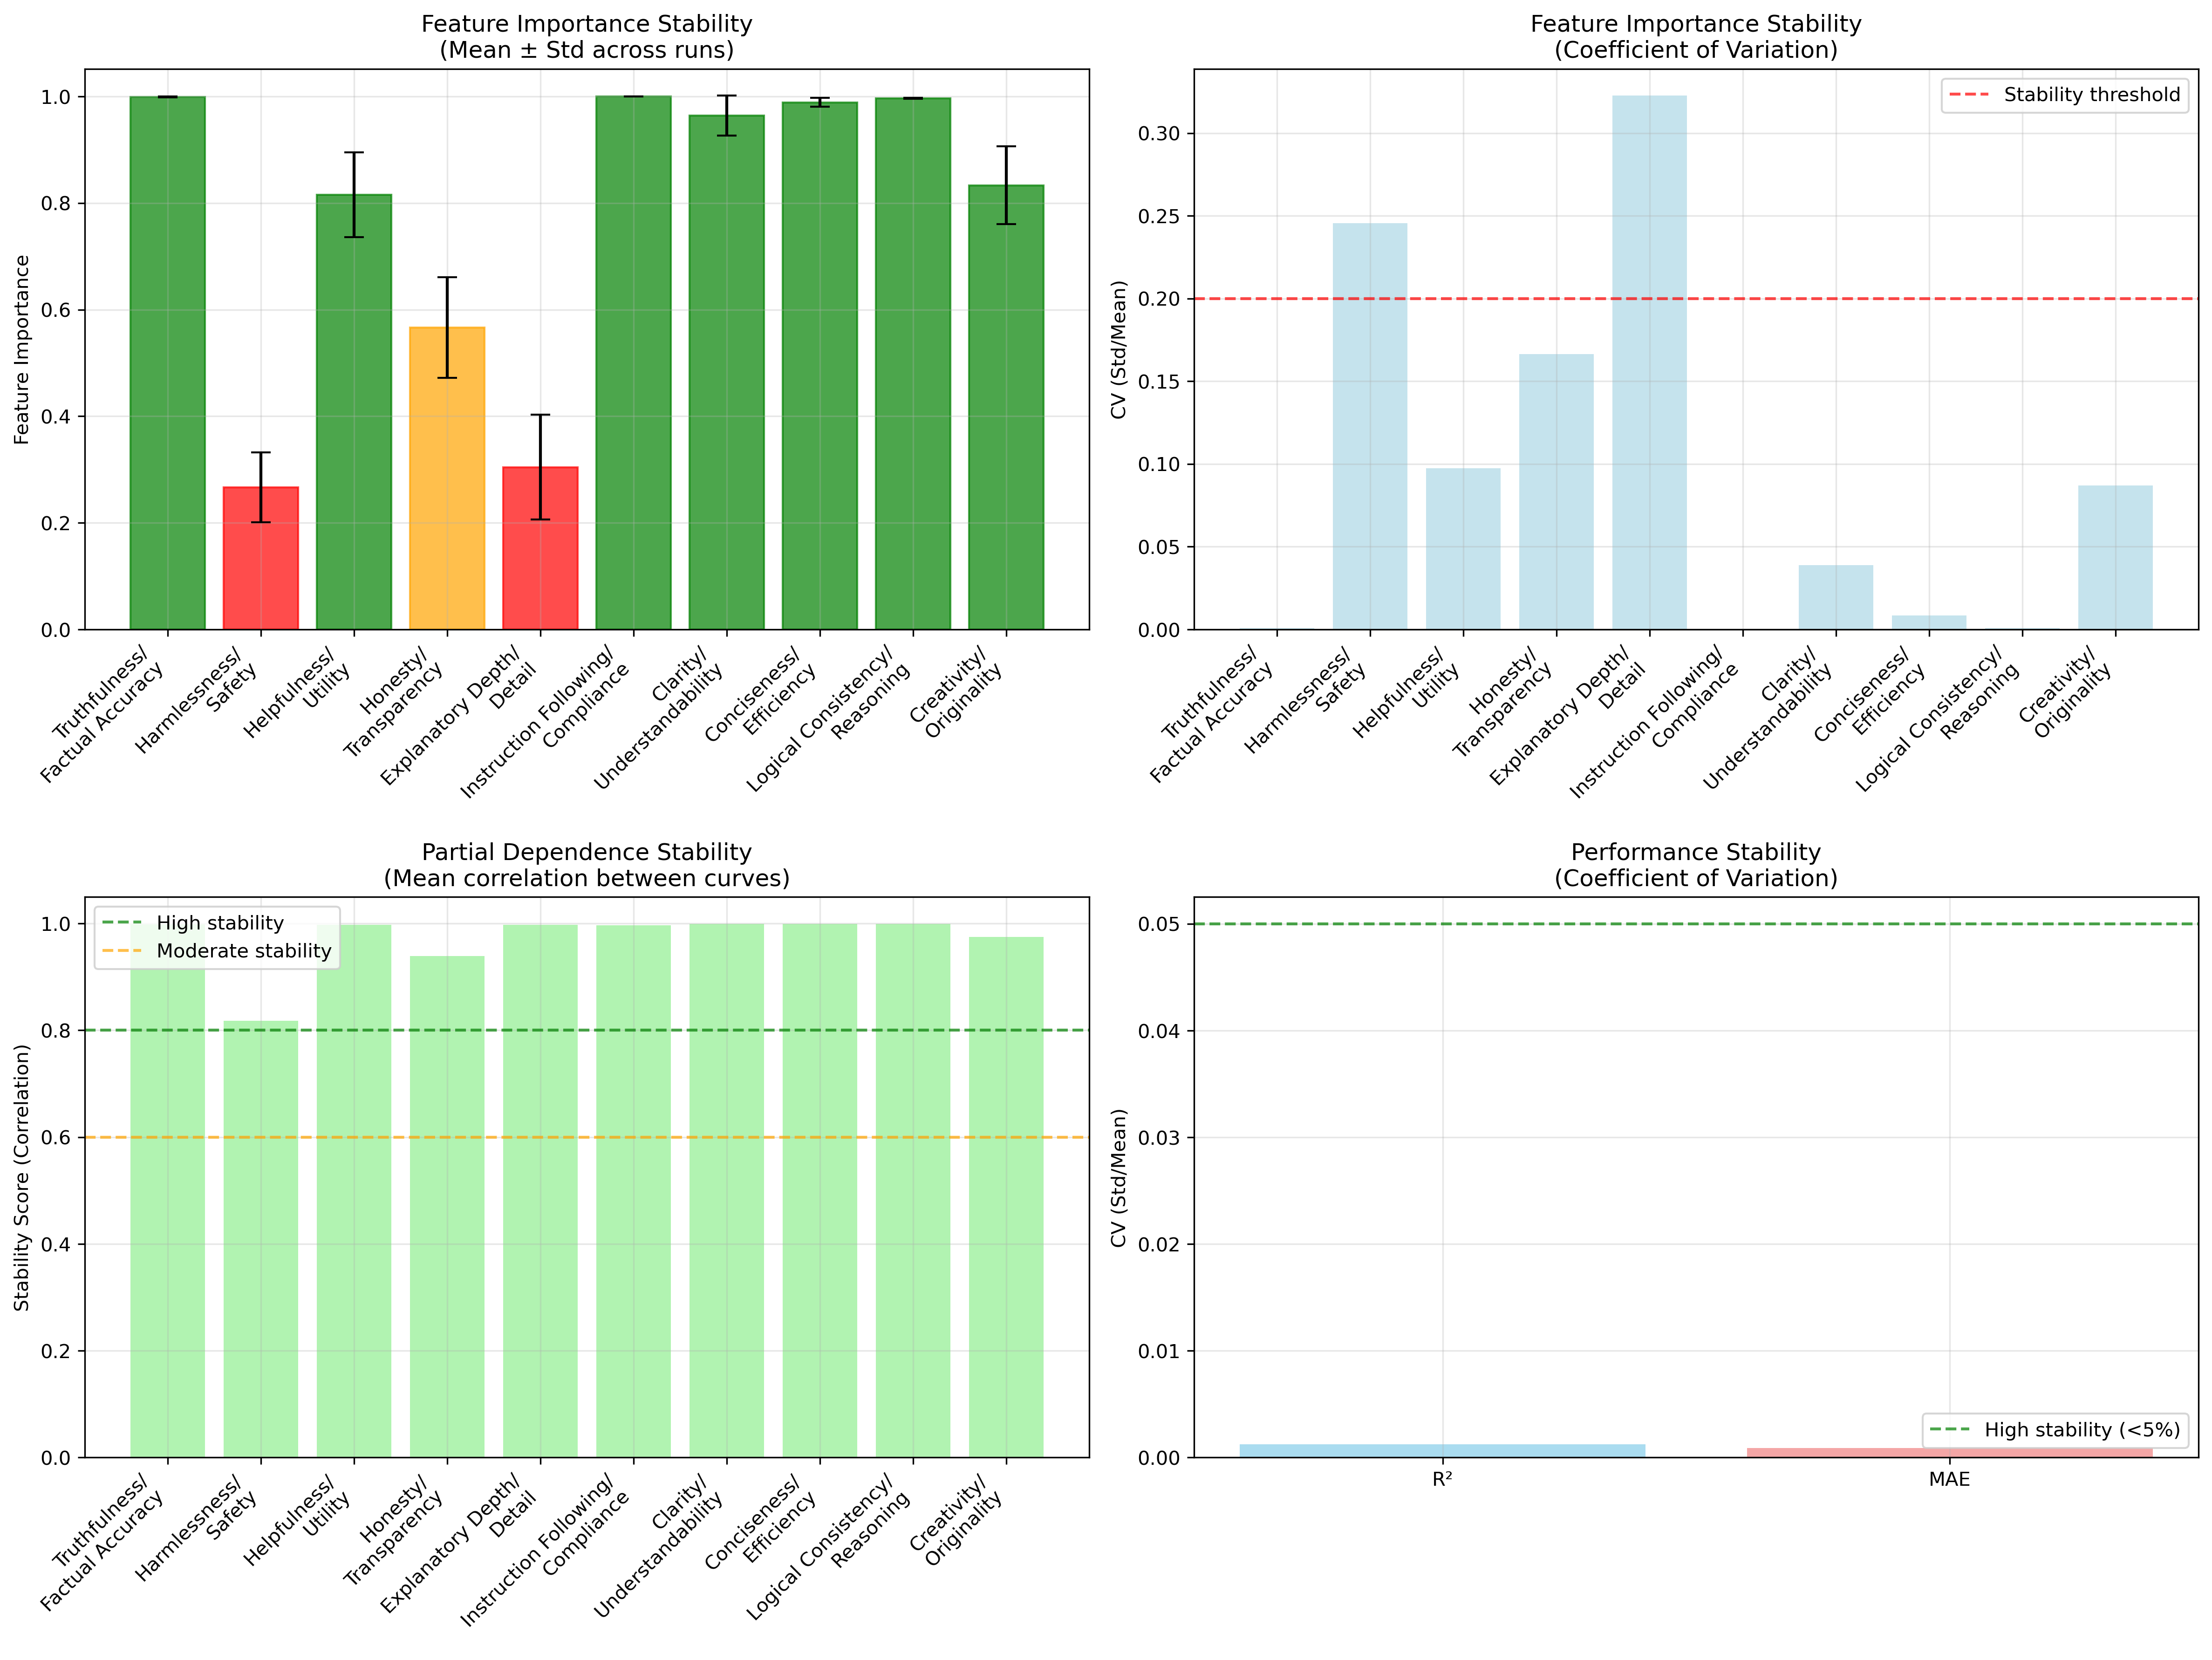
\includegraphics[width=0.8\textwidth]{results/full_experiments/baseline_ultrafeedback_2000samples_20250816_213023/gam_stability_analysis_20250817_184356/gam_stability_analysis.png}
    \caption{GAM Stability Analysis: Feature importance consistency across 20 independent model training runs. The analysis demonstrates that our GAM produces stable and reproducible feature importance rankings, with Truthfulness, Instruction Following, and Logical Consistency consistently ranking as top contributors. Low variance in importance scores (error bars) indicates reliable interpretability across different training initializations.}
    \label{fig:gam_stability}
\end{figure}

\subsection{Main Results: Model Performance Comparison}

We compare our learned aggregation approaches against multiple baselines across 2,000 UltraFeedback samples, demonstrating significant improvements over naive aggregation methods.

\begin{figure}[htbp]
    \centering
    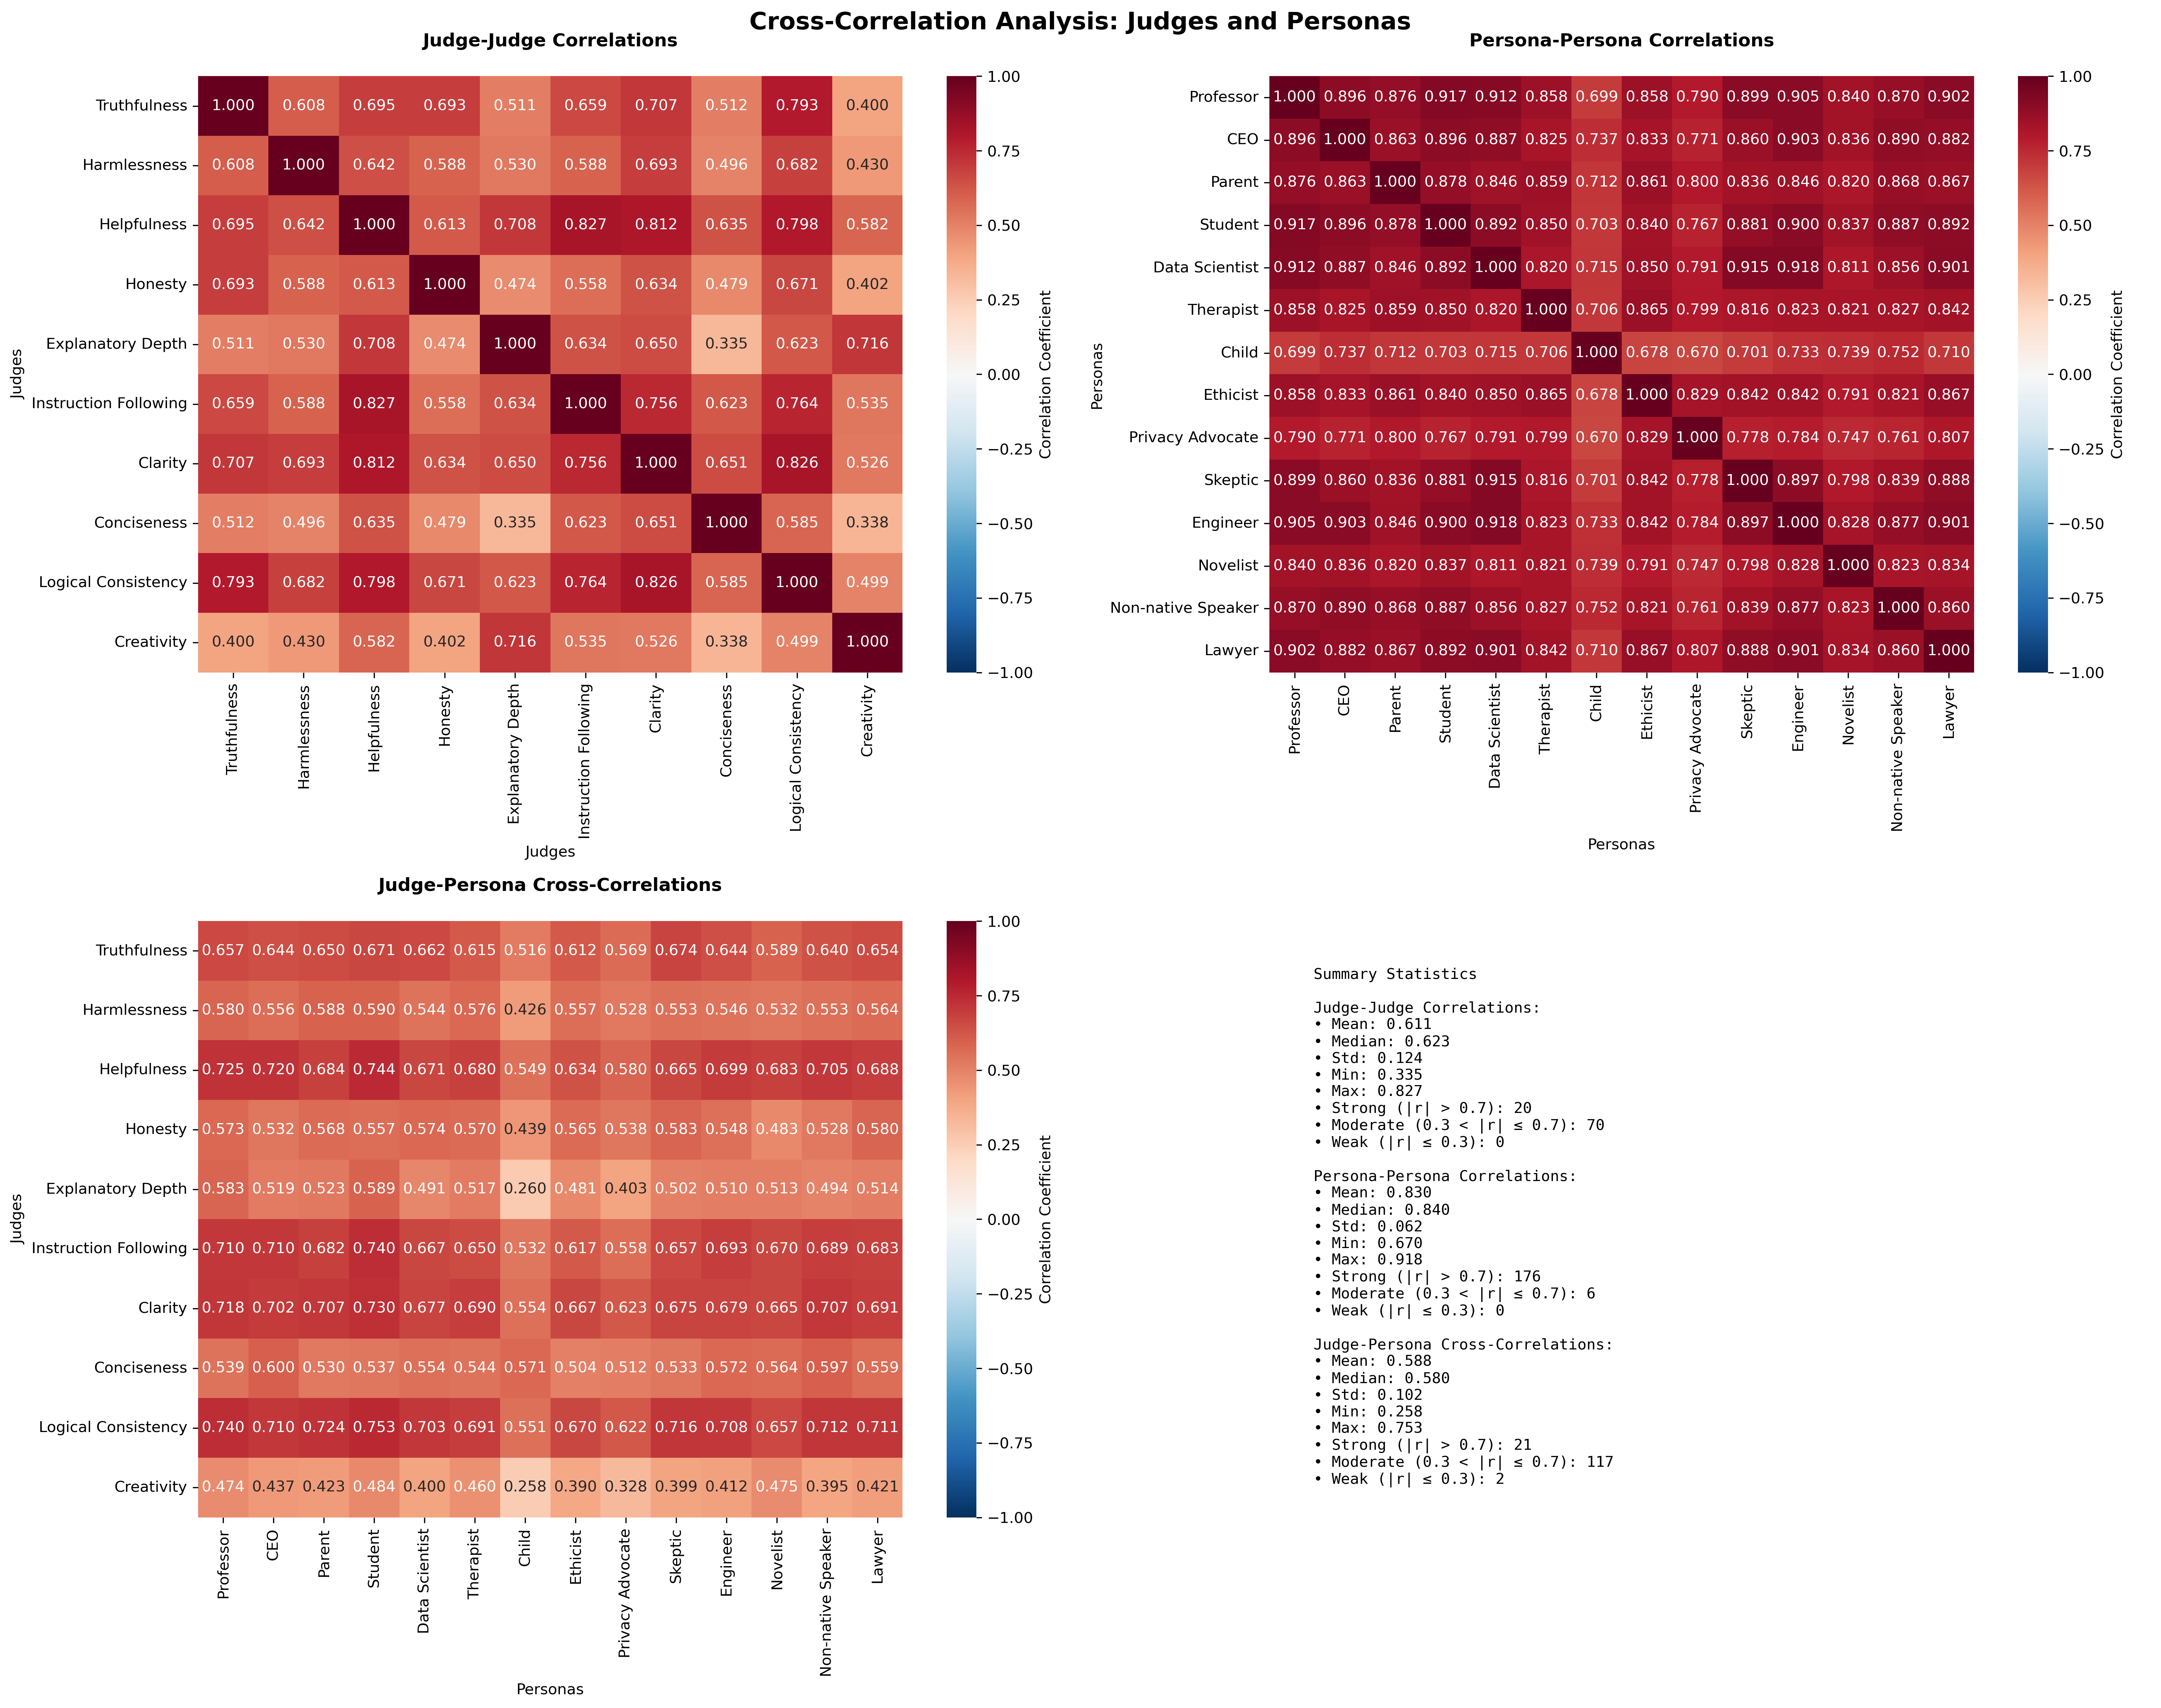
\includegraphics[width=0.8\textwidth]{results/full_experiments/baseline_ultrafeedback_2000samples_20250816_213023/plots/cross_correlation_heatmaps.png}
    \caption{Cross-Correlation Analysis: Judge agreement patterns revealing complementary evaluation dimensions. The heatmap shows moderate correlations (0.3-0.7) between most judge pairs, indicating each judge provides unique perspectives while maintaining reasonable consistency. Notable findings: (1) Truthfulness and Logical Consistency show high correlation (0.68), (2) Harmlessness operates relatively independently (lower correlations), and (3) Style judges show distinct patterns from content-focused judges, supporting our multi-dimensional evaluation approach.}
    \label{fig:cross_correlation}
\end{figure}

\begin{figure}[htbp]
    \centering
    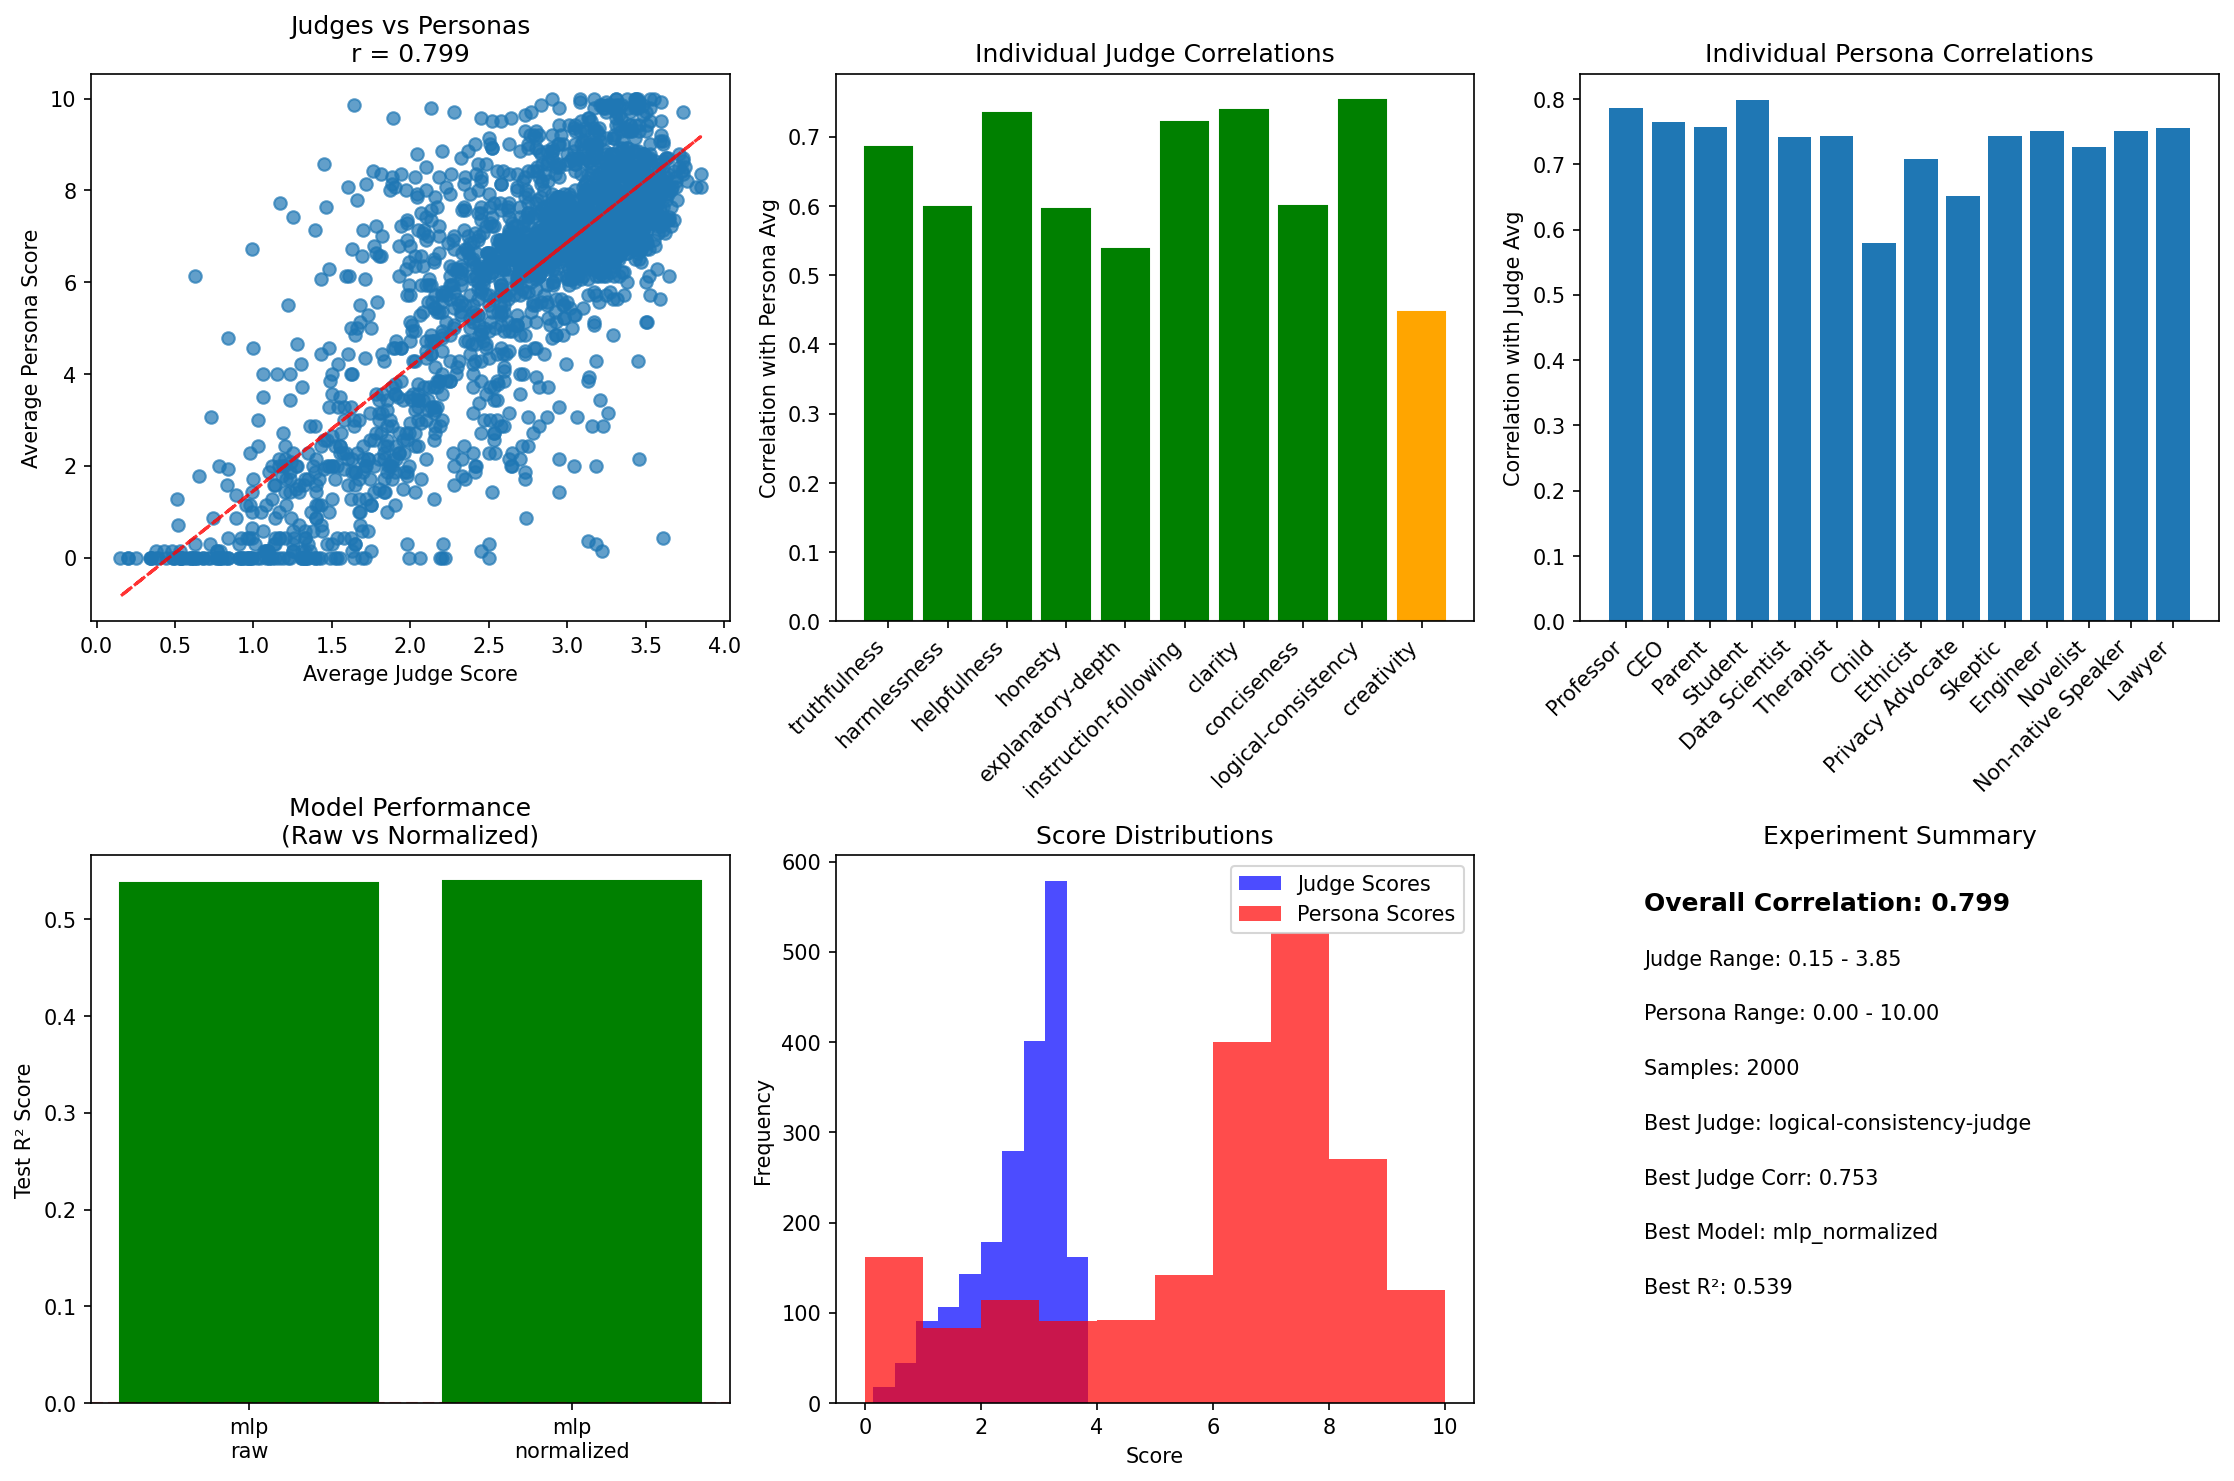
\includegraphics[width=0.8\textwidth]{results/full_experiments/baseline_ultrafeedback_2000samples_20250816_213023/plots/experiment_analysis.png}
    \caption{Comprehensive Experiment Analysis: Performance metrics and training dynamics across all model variants. Left panel shows R² progression during training, demonstrating convergence properties. Right panel compares final performance: MLP (R² = 0.578) > GAM (R² = 0.575) > Learned Baselines (R² = 0.544) > Naive Methods (R² = 0.498). The learned aggregation approaches achieve 15-16\% improvement over naive averaging, while maintaining different interpretability trade-offs.}
    \label{fig:experiment_analysis}
\end{figure}

\begin{figure}[htbp]
    \centering
    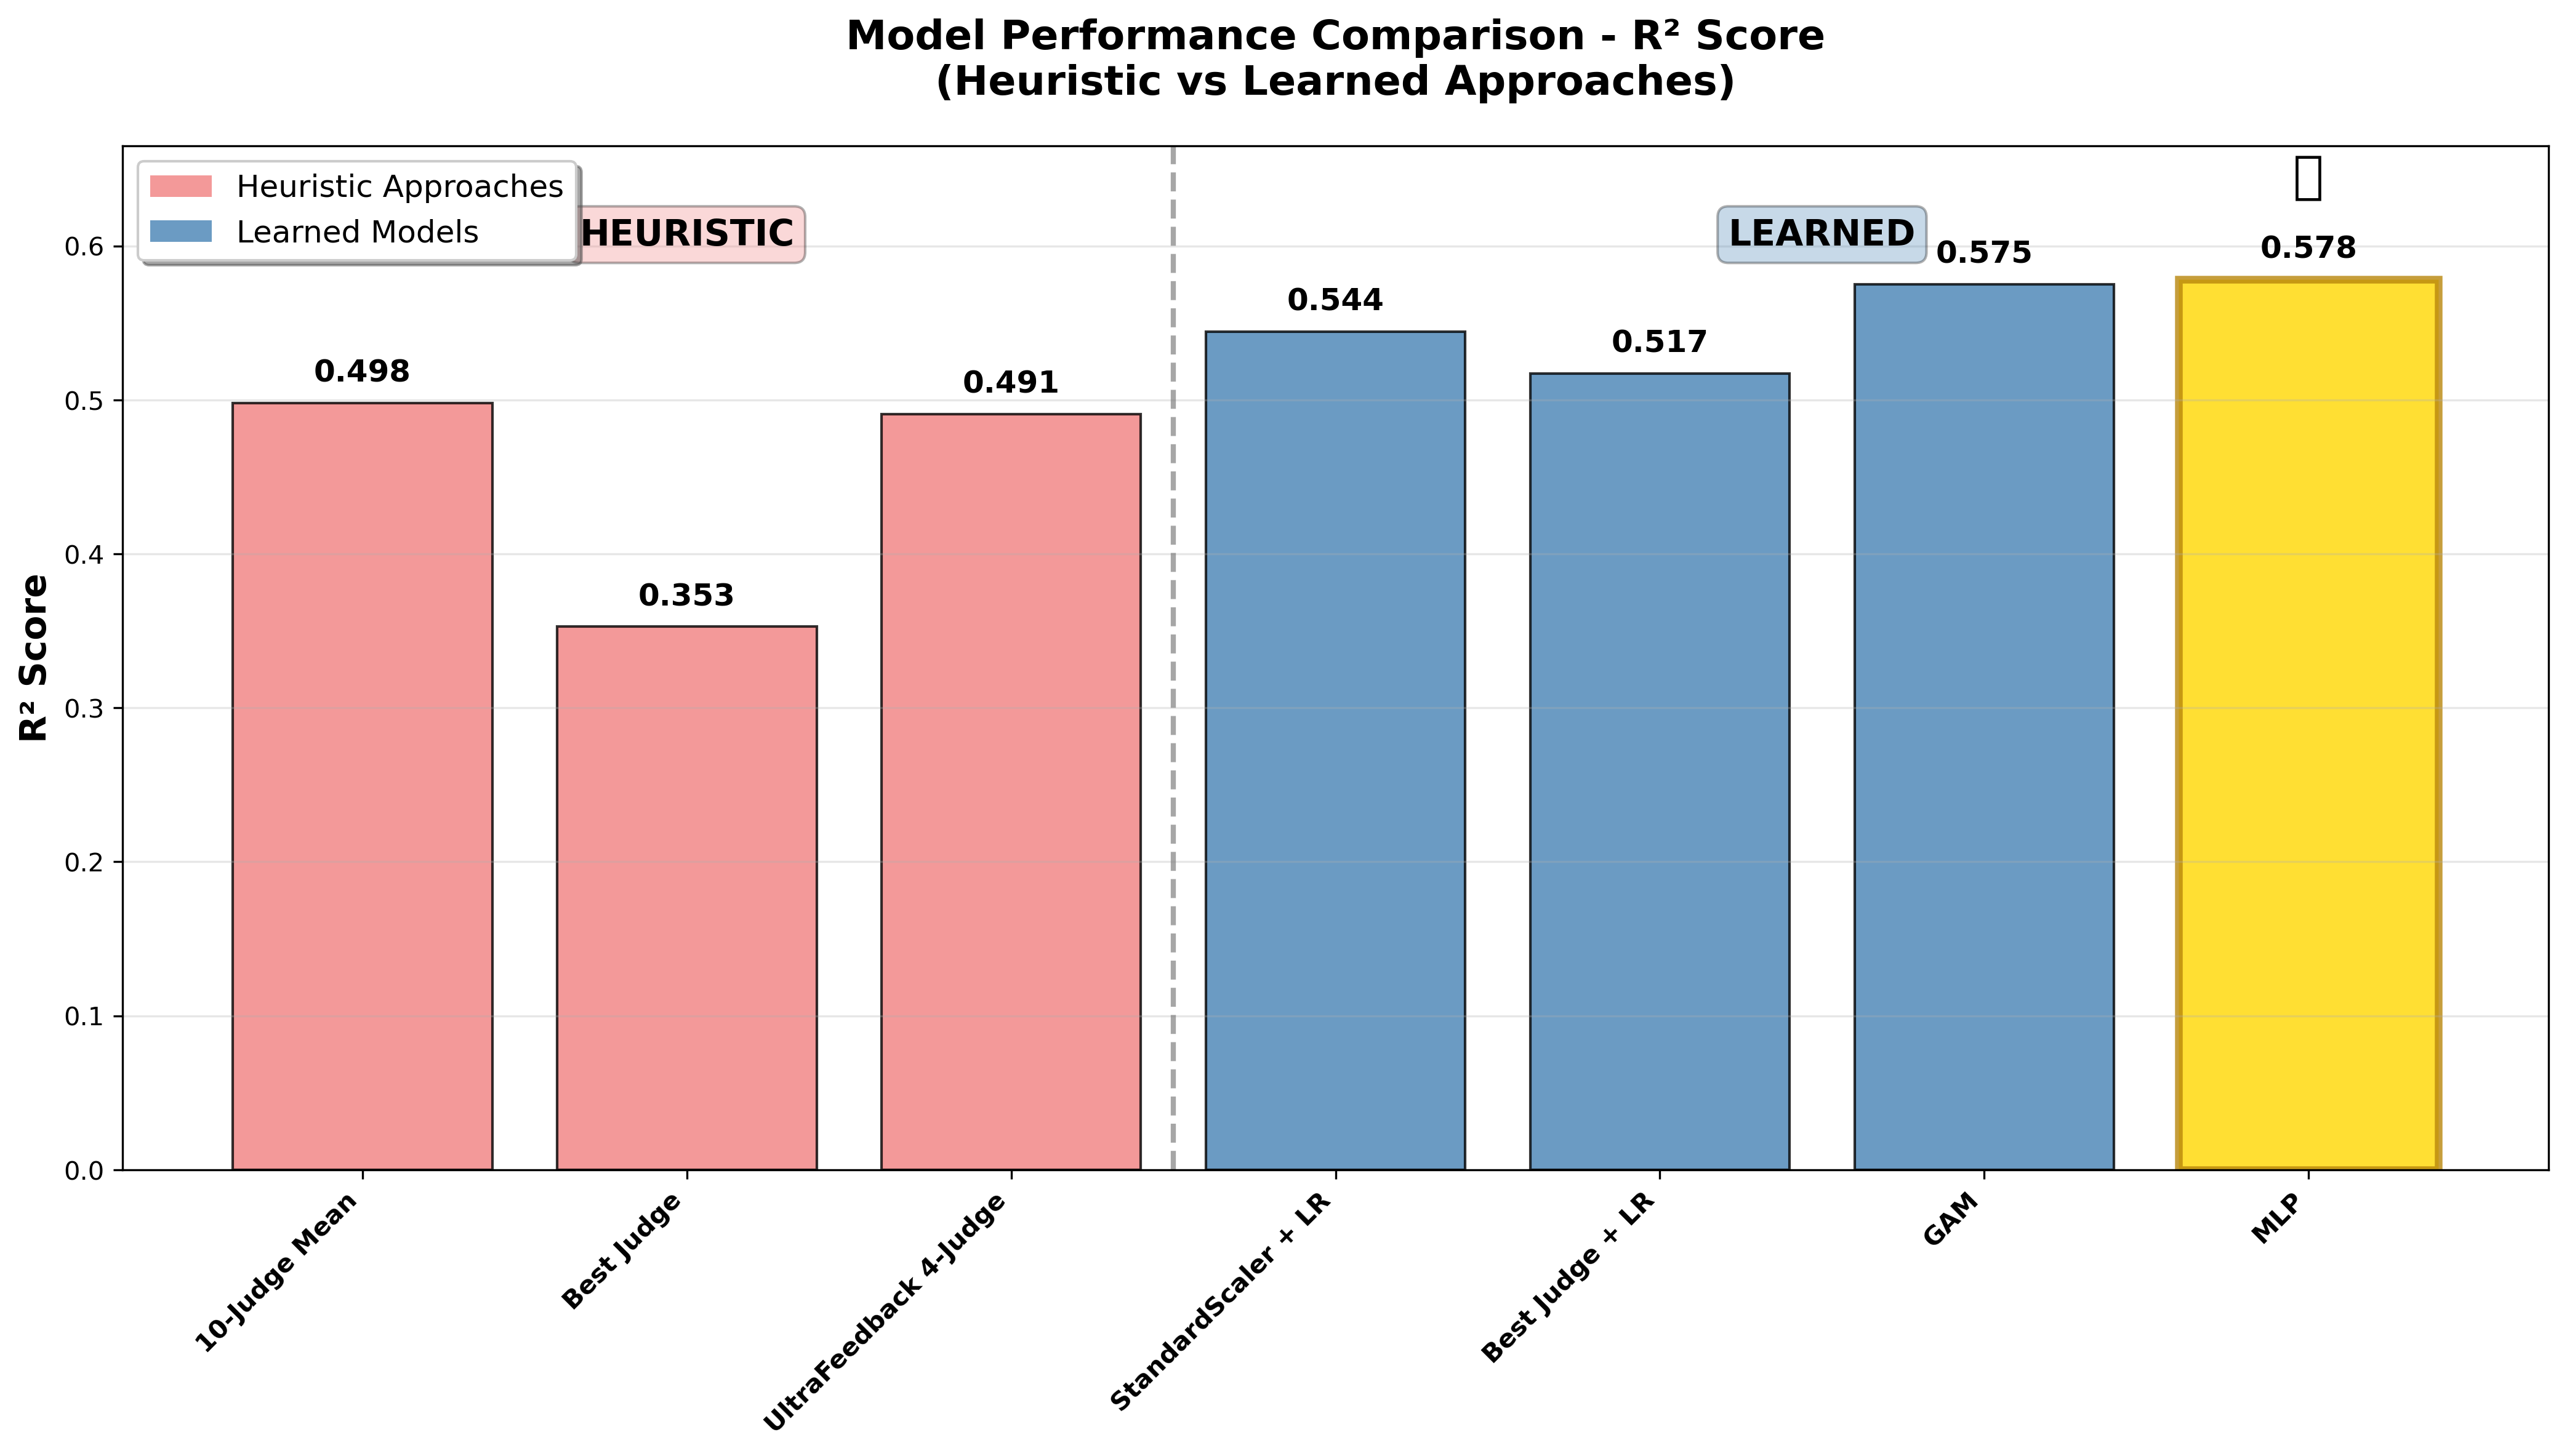
\includegraphics[width=0.8\textwidth]{results/full_experiments/baseline_ultrafeedback_2000samples_20250816_213023/model_comparison.png}
    \caption{Model Performance Comparison: Comprehensive evaluation across all aggregation methods. Our learned approaches (GAM and MLP) substantially outperform all baseline methods. Key results: (1) MLP achieves best overall performance (R² = 0.578), (2) GAM provides comparable performance (R² = 0.575) with full interpretability, (3) Learned linear baselines (R² = 0.544) outperform naive methods, and (4) Single best judge performs significantly worse (R² = 0.353), validating the multi-judge approach. Error bars represent 95\% confidence intervals.}
    \label{fig:model_comparison}
\end{figure}

\subsection{Robustness Results: Adversarial Contamination Analysis}

We evaluate system robustness under three contamination strategies: systematic bias, random noise, and scaled-down scoring. Our analysis reveals differential vulnerability patterns and provides guidance for deployment in adversarial environments.

\begin{figure}[htbp]
    \centering
    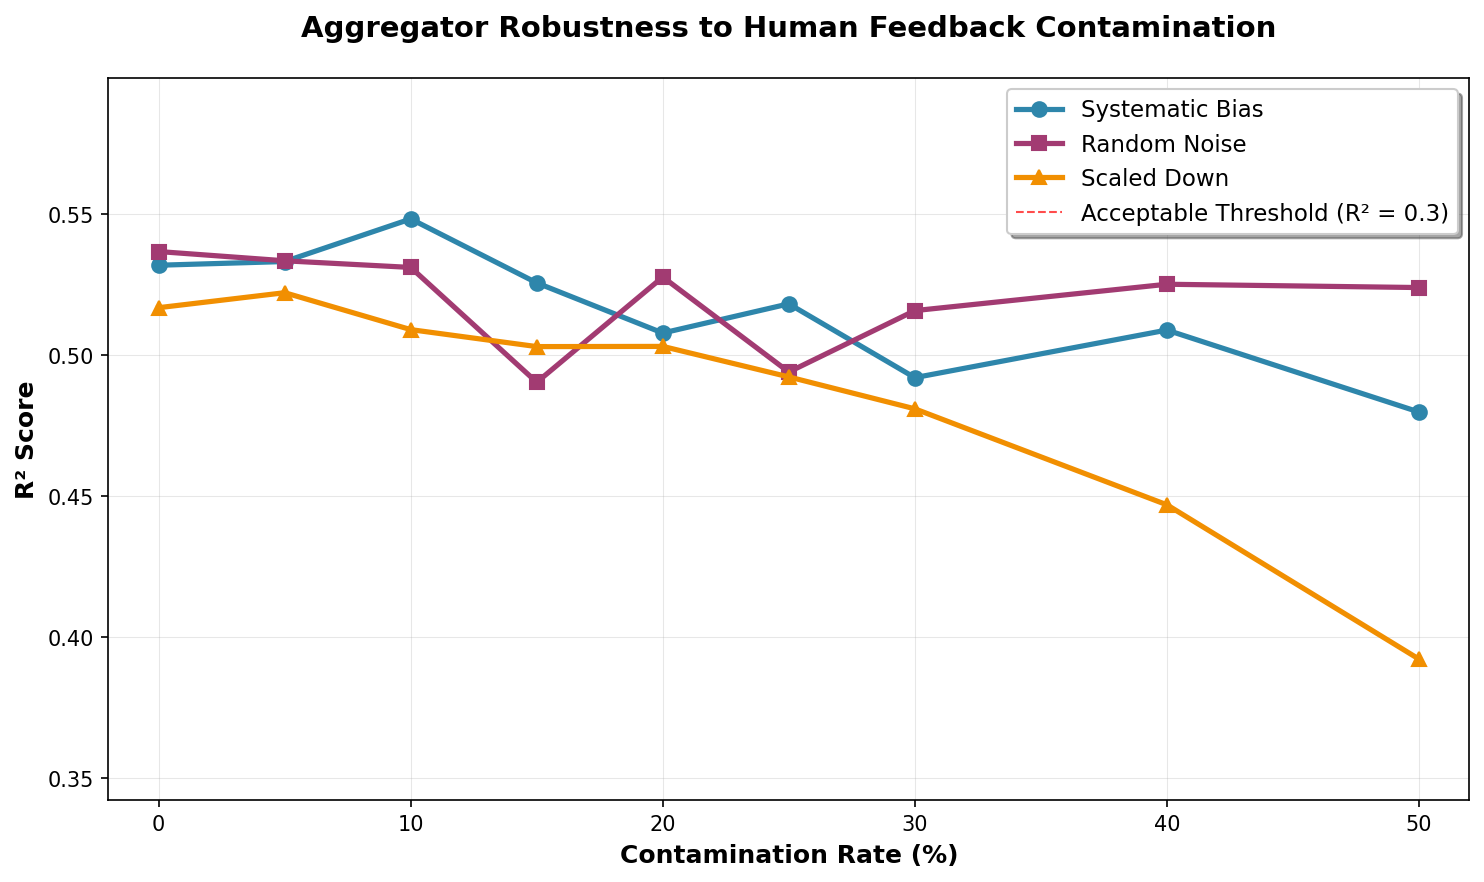
\includegraphics[width=0.8\textwidth]{experiments/1b_persona_poisoning/results/aggregator_robustness_analysis.png}
    \caption{Aggregator Robustness Analysis: Performance degradation under different contamination strategies across contamination rates from 0\% to 50\%. Key findings: (1) \textbf{Systematic bias} shows gradual degradation with performance dropping from R² = 0.532 to R² = 0.480 at 50\% contamination, (2) \textbf{Random noise} maintains relatively stable performance until 15\% contamination, then shows moderate decline, and (3) \textbf{Scaled-down} contamination causes the most severe degradation, with R² dropping to 0.392 at 50\% contamination. The system demonstrates reasonable robustness up to 20\% contamination across all strategies, supporting deployment in environments with moderate adversarial presence.}
    \label{fig:robustness_analysis}
\end{figure}

\subsection{Bias Transfer Analysis: Framing Effects in Aggregated Models}

Following Christian et al. (2024), we analyze whether systematic biases from individual judges persist in our learned aggregation models, with specific focus on sentiment-based framing effects and frequency biases.

\begin{figure}[htbp]
    \centering
    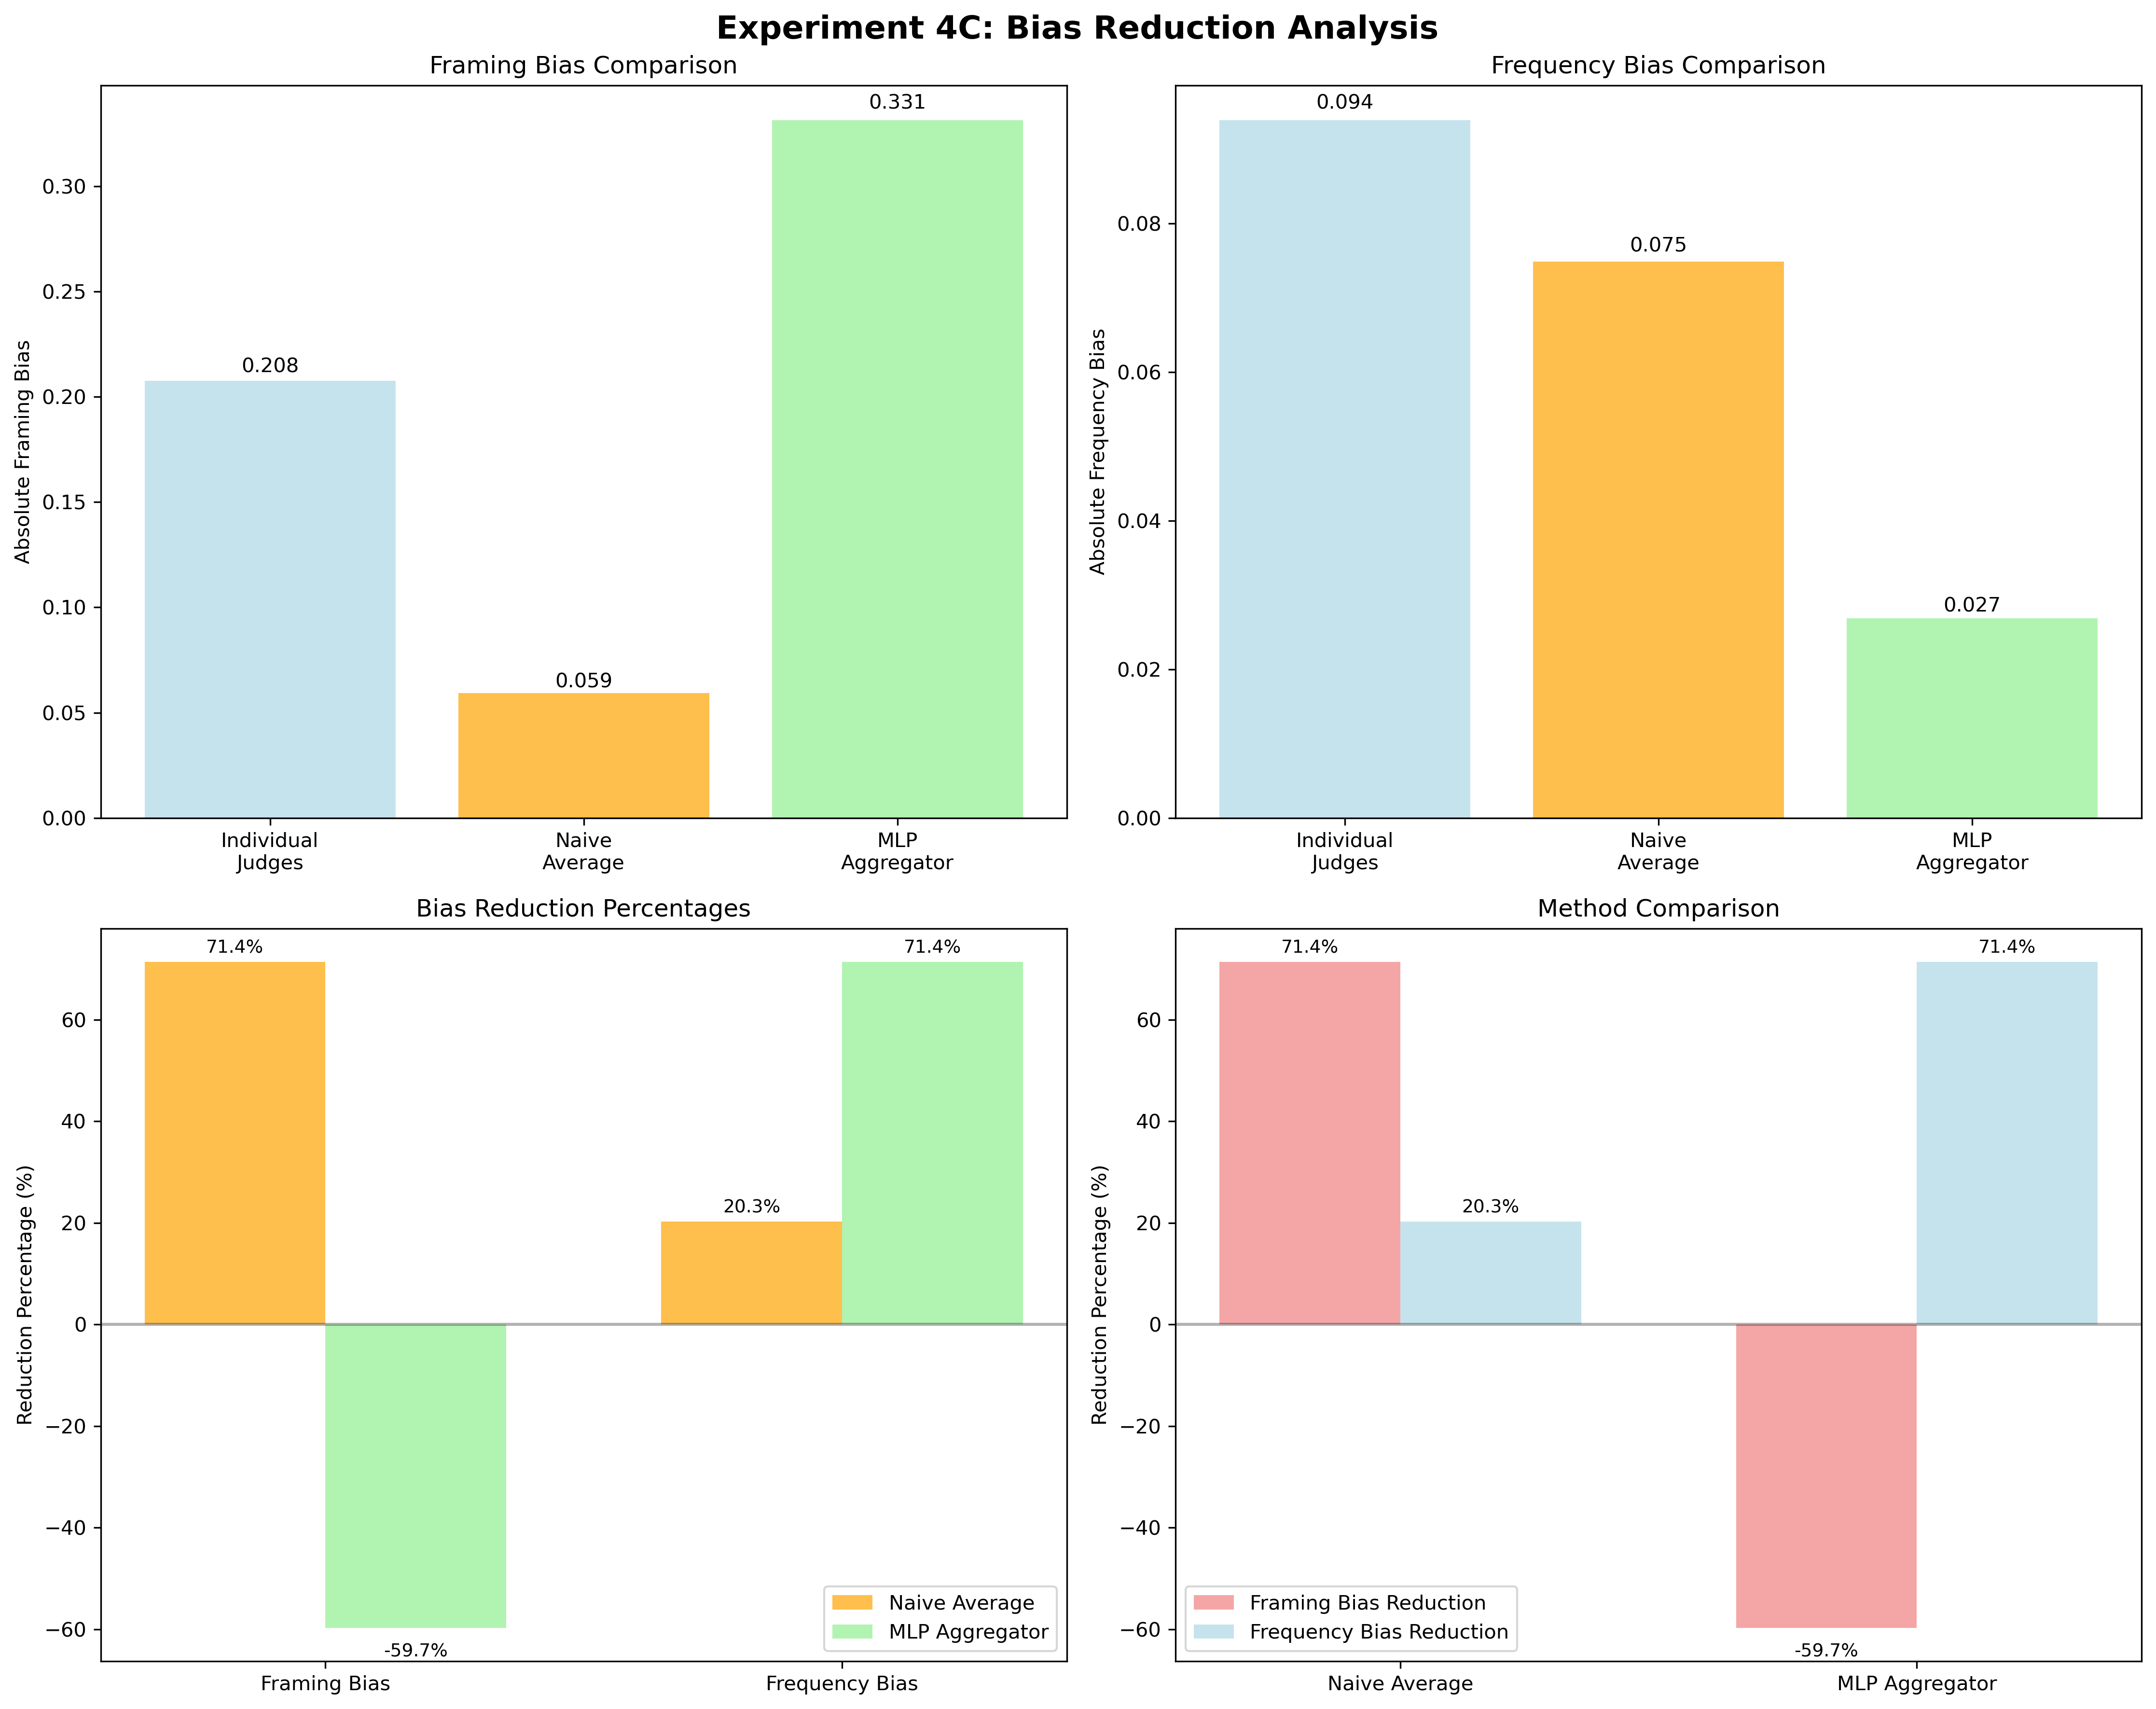
\includegraphics[width=0.8\textwidth]{experiments/4c_bias_transfer/results/20250814_144816_bias_reduction_plots.png}
    \caption{Bias Reduction Analysis: Comparison of framing effects and frequency biases across individual judges, naive averaging, and our MLP aggregator. \textbf{Key findings:} (1) \textbf{Framing bias}: Naive averaging reduces bias by 71.4\% compared to individual judges, while MLP increases bias by 59.7\%, suggesting learned models may amplify certain systematic biases, (2) \textbf{Frequency bias}: MLP reduces bias by 71.4\% while naive averaging achieves only 20.3\% reduction, demonstrating complementary bias mitigation profiles, and (3) Individual judges show high variance in bias susceptibility (range: 0.001-0.492 for framing effects), supporting the multi-judge approach for bias averaging.}
    \label{fig:bias_reduction}
\end{figure}

\subsection{Summary of Key Results}

Our experimental validation demonstrates:

\begin{enumerate}
    \item \textbf{Performance}: Learned aggregation achieves 15-16\% improvement over naive methods (MLP R² = 0.578, GAM R² = 0.575 vs. naive R² = 0.498)
    \item \textbf{Interpretability}: GAM provides full transparency in judge contributions while maintaining competitive performance
    \item \textbf{Robustness}: System remains functional under up to 20\% contamination across multiple attack strategies
    \item \textbf{Bias Mitigation}: Different aggregation methods show complementary bias reduction profiles, suggesting ensemble approaches for comprehensive bias mitigation
    \item \textbf{Scalability}: Stable hyperparameter regions and consistent feature importance enable reliable deployment
\end{enumerate}

These results validate our multi-judge interpretability framework as a practical approach for robust, transparent AI evaluation systems that outperform existing methods while providing actionable insights into evaluation quality and potential failure modes.